\documentclass[a4paper,12pt,onesided]{report}
%Eigene Änderungen:
\usepackage{cite}
\usepackage[addtotoc]{abstract} %mit hinzufügen ins inhaltsverzeichnis
\usepackage[utf8]{inputenc}

%===========================================================
%== Definitionen fuer die Formatierung =====================
%===========================================================

% Use german names like "Literaturverzeichnis" instead of "Bibliography"
\usepackage{ngerman}

% Links inside of the document
%\usepackage{hyperref}

% Allows to use graphics
\usepackage{graphicx}

% Use times new roman and courier as fonts
\usepackage{times}
\usepackage{courier}

% Allow forcing positioning of floating figures
\usepackage{float}

% Allow special tye of configurable tables
\usepackage{tabularx}
\usepackage{multirow}


% Allows to change letter spcaing
\usepackage{microtype}

% Special table types
\usepackage{longtable}
\usepackage{colortbl}
\definecolor{gray}{gray}{0.85}


\usepackage[titles]{tocloft}


\usepackage{url}

\usepackage{listings}
\renewcommand*{\lstlistlistingname}{Codebeispielverzeichnis}
\renewcommand{\lstlistingname}{Code}
\lstset{frame=single,basicstyle=\footnotesize\bfseries\ttfamily,breaklines=true}

\usepackage{titlesec}
\titlespacing*{\chapter}{0pt}{-35pt}{0pt}

\lstset{numberbychapter=false}
\usepackage{chngcntr}
\counterwithout{figure}{chapter}
\counterwithout{table}{chapter}
\renewcommand{\tablename}{Tab.}

% Glossary
% More info here https://en.wikibooks.org/wiki/LaTeX/Glossary
\usepackage[toc]{glossaries}
\renewcommand*{\glossaryentrynumbers}[1]{}
\makeglossaries

% Some formatting stuff for "Praxisbericht"
\linespread{1.4}
\makeatletter
 \renewcommand*\l@section{\@dottedtocline{1}{0em}{2.3em}}
 \renewcommand*\l@subsection{\@dottedtocline{1}{1em}{2.3em}}
\makeatother
\usepackage[a4paper, left=2.5cm, right=2.5cm, top=2.5cm, bottom=2.5cm]{geometry}

\usepackage{fancyhdr}
\pagestyle{fancy}
\fancyfoot{}
\fancyfoot[R]{\thepage}
\fancyhead{}
\fancyhead[L]{\nouppercase{\leftmark}}
\fancypagestyle{plain}{\pagestyle{fancy}}



% for formatting titles of chapters
\usepackage{titlesec}

\titleformat{\chapter} % command
{\bfseries} % format
{\fontsize{16}{18}\selectfont \thechapter\ } % label
{0ex} % sep
{\fontsize{16}{18}\selectfont} % before-code
[] % after-code
\titleformat{\section} % command
{\bfseries} % format
{\fontsize{14}{16}\selectfont \thesection\ } % label
{0ex} % sep
{\fontsize{14}{16}\selectfont} % before-code
[] % after-code
\titleformat{\subsection} % command
{\bfseries} % format
{\fontsize{12}{14}\selectfont \thesubsection\ } % label
{0ex} % sep
{\fontsize{12}{14}\selectfont} % before-code
[] % after-code
 
% Linksbuendige Captions
\usepackage{caption}
\captionsetup{
  justification=raggedright,
  singlelinecheck=false
}

% Paragraph styles
\setlength{\parindent}{0cm}
\setlength{\parskip}{6pt}

% A todo macro for marking ToDos
\usepackage{color}
\newcommand{\todo}[1]{\textcolor{white}{\colorbox{red}{ To do %
       :}}\textcolor{red}{\ \ #1
   }\textcolor{red}{\colorbox{red}{III}}\ }




\begin{document}

% Titelseite
\begin{titlepage}
	\centering
	
\includegraphics[width=14.9cm]{img/logo}\\

	\fontsize{18}{20}\selectfont
	Hochschule für angewandte Wissenschaften Coburg\\[.1cm]
	Fakultät Elektrotechnik und Informatik\\[1.2cm]
	Studiengang: Informatik\\
	Bachelorarbeit\\[1.2cm]
	\fontsize{21}{23}\selectfont
	\textbf{Entwicklung einer hardwarebeschleunigten Berechnung der 
	Mandelbrotmenge auf einem FPGA}\\[1cm]
	\fontsize{18}{20}\selectfont
	von\\[1.2cm]
	Daniel Kirchner\\
	Matrikelnummer: 02219415\\[1.2cm]
	Abgabe der Arbeit: 15.07.2019\\[1.2cm]

	Betreut durch: Prof. Oliver Engel, Hochschule Coburg
\end{titlepage}

\begin{abstract}
	Im Rahmen dieser Bachelorarbeit wurde eine hardwarebeschleunigte Visualisierung der Mandelbrotmenge auf einem FPGA realisiert.
	Hierfür werden diverse mathematische und designtechnische Performanceoptimierungen vorgestellt, welche dann in einparalleles FPGA-Design implementiert wurden. Weiterhin sollen einige Eigenschaften und Besonderheiten der Mandelbrotmenge und von Fraktalen im Allgemeinen aufgezeigt werden.\\
	Das Projekt wurde für das Zybo Zynq-7000 Trainer Board entwickelt, welches über einen VGA-Output die Repräsentation des Fraktals in Form eines 800x600@60Hz Videosignals ausgibt. Zur optimalen Ausnutzung der auf diesem Board gegebenen Ressourcen (DSPs, BRAM) wurde die \textit{Vivado Design Suite} mit dem integrierten IP-Katalog verwendet.\\

	%TODO: englisch
\end{abstract}

% Inhaltsverzeichnis
{
  \setlength{\cftbeforechapskip}{-.5ex}
  \tableofcontents
  \addcontentsline{toc}{chapter}{Inhaltsverzeichnis}
}

% Abbildungsverzeichnis
\newpage
\listoffigures
\addcontentsline{toc}{chapter}{Abbildungsverzeichnis}

% Tabellenverzeichnis
\newpage
\listoftables
\addcontentsline{toc}{chapter}{Tabellenverzeichnis}

% Codeverzeichnis
\newpage
\lstlistoflistings
\addcontentsline{toc}{chapter}{Codebeispielverzeichnis}

% Abkuerzungsverzeichnis
\newpage
\section*{Abkürzungsverzeichnis}
\addcontentsline{toc}{chapter}{Abkürzungsverzeichnis}
\begin{tabular}{ll}
  JAX-RS&Java API for RESTful Web Services\\
  % TODO: updaten
\end{tabular}

% Beginn Arbeit
\newpage
\chapter{Einleitung}

%TODO vllt aufbau erklären
\section{Motivation}
Die stets wachsende Zahl von Komponenten die auf einem mikroelektronischen Bauteil pro Zeiteinheit untergebracht wird, ist ein Phänomen, welcbes Gordon Moore schon im Jahr 1965 aufgefallen ist \cite{moore1965cramming}. Die populäre, nach ihm benannte Beobachtung, dass die Anzahl der Transistoren pro integriertem Schaltkreis exponentiell mit der Zeit ansteigt ist allgemein als das Mooresche Gesetz bekannt.

Diese Gesetzlichkeit machte es möglich den stets wachsenden Leistungsanforderungen an moderne Hardware gerecht zu werden, indem immer mehr (und komplexere) identische Allzweck-Prozessoren (Kerne) pro CPU verbaut wurden.

Dieses Vorgehen kann jedoch nicht unbegrenzt lange betrieben werden, da die heute verwendeten MOS-Transistoren sich rapide ihren physikalischen Grenzen annähern. Ein besserer Umgang mit dem stetig steigenden Bedarf an Rechenleistung ist die Entwicklung von spezialisierter Hardware, welche zwar nur ein kleines Aufgabenspektrum abdeckt, dies jedoch mit hoher Performanz und Energieeffizienz tut.

Ein Beispiel hierfür ist die moderne Grafikkarte (GPU), welche dem Prozessor Darstellungsberchnungen abnimmt, wodurch dieser mehr Zeit hat, andere Aufgaben zu übernehmen. Die Grafikkarte führt diese Aufgaben mit enorm hohem Durchsatz und niedrigen Berechnungszeiten durch, welche ein herkömmlicher Prozessor alleine nicht erreichen könnte.

Auch andere Hardwarekomponenten, wie die Netzwerkkarte, kryptographische Beschleuniger, oder Soundkarten sind in fast allen Computersystemen verbaut und entlasten den Hauptprozessor. Man spricht auch von heterogenen Computersystemen.

Die im Rahmen dieser Arbeit vorgestellte Hardware soll ein Beispiel für eine derartige heterogene Komponente sein. Auf einem Field Programmable Gate Array (FPGA) %TODO Kapitel linken
soll eine performante und energieffiziente Visualisierung der sogenannten Mandelbrotmenge realisiert werden. Diese Problemstellung ist auch durch einen ordinären Prozessor lösbar, lastet diesen jedoch enorm aus und ist somit auch sehr energieineffizient. %TODO Kapitel linken

\section{Aufgabenstellung}
Die Aufgabe dieses Projektes ist es, eine komplett in Hardware stattfindende Berechnung der Mandelbrotmenge durchzuführen und die Ergebnisse über eine VGA-Schnittstelle darzustellen (ähnlich Bild) %TODO
%TODO Mandelbrotmenge Bild

Weiterhin soll die Hardware durch externe Peripherie konfigurierbar hinsichtlich der angestellten Berechnungen sein. So soll etwa aktuell abgebildete Bereich der Mandelbrotmenge oder auch die Farbgebung der Darstellung im laufenden Betrieb geändert werden können.

Hierfür wurde das FPGA-Trainer Board \textit{Zybo Zynq-7000} zur Verfügung gestellt, welches in %TODO Kapitel linken
genauer vorgestellt wird.

\section{Mitgelieferte Skripte}
%TODO: github repository
Im Git-Repository ... sind sämtliche Python-Skripts, die zur Erstellung von selbsterstellten Bildern verwendet wurden, enthalten. Des weiteren gibt die dort enhaltene Datei \textit{readme.md} Aufschluss über nützliche Skripts, die im Rahmen dieser Arbeit verwendet wurden.

\chapter{Technische Grundlagen}
Zum besseren Verständnis des Gesamtprojektes sollen in diesem Kapitel einige technische Konzepte erläutert werden.

\section{FPGAs}
Ein \textit{Field Programmable Gate Array} (kurz FPGA) ist ein Schaltkreis, welcher mit Hilfe von Hardwarebeschreibungssprachen %TODO Kapitel
konfiguriert werden kann, um beliebig komplexe logische Schaltungen zu realisieren.\\
Das Grundelement eines solchen Bausteines bilden die sogenannten \textit{Lookup Tables} (kurz LUTs), welche zu einem beliebigen n-bit Input ein 1-bit Output Signal produzieren. Die zugrundeliegende Logiktabelle einer LUT ist hierbei frei programmierbar.

\begin{figure}[H]
	\centering
	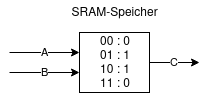
\includegraphics{LUT.png}
	\caption{Beispielhafter Aufbau einer 2-Input LUT}
	\label{fig:LUT}
\end{figure}

Eine LUT, welche die Operation $C = A \oplus B$ implementiert ist in \autoref{fig:LUT} zu sehen. In dieser wird in einem SRAM-Speicher für jede Inputkombination ein Outputwert hinterlegt, wodurch jede 2-Bit Funktion abgebildet werden kann. In Verbindung mit einem Flipflop \footnote{Ein Flipflop ist ein Speicherelement, welches einen einzigen Bit Daten halten kann.} bildet eine LUT dann einen sogenannten Logikblock (s. \autoref{fig:logikblock}).\cite{fpgaDesign}

\begin{figure}[H]
	\centering
	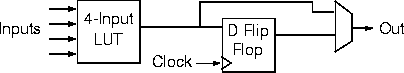
\includegraphics{logic_block.png}
	\caption{Logikblock, aus \cite{fpgaDesign}}
	\label{fig:logikblock}
\end{figure}

Ein FPGA verbindet nun durch ebenfalls konfigurierbare Bussysteme viele solcher Logikblöcke um komplexere Schaltkreise abzubilden.\\
Weiterhin verfügen FPGA-Boards oft noch über ergänzende Hardwarekomponenten, von denen die im Falle dieses Projektes vorhandenen im Folgenden gezeigt werden sollen.

\paragraph{DSP}
Ein \textit{Digitaler Signalprozessor} (DSP) ist ein fest integrierter Baustein, welcher durch Multiplizierer und Akkumulatoren binäre Algorithmen beschleunigt.
So übernimmt dieser etwa grundlegende mathematische Operationen, was dazu führt, dass diese flächen- und energiesparender durchgeführt werden, als bei der Verwendung von LUTs \cite[S. 52]{dsps}.
Typische Anwendungsgebiete dieser Bausteine sind Fließkommamultiplikationen, Schnelle Fourier-Transformationen oder einfache Zähler \cite[S. 14]{dsps}. 
In diesem Projekt wurden die DSPs hauptsächlich aufgrund ihrer 25x18 Bit Multiplizierer verwendet, welche kaskadiert werden können um beliebig Breite Multiplikationen durchzuführen.

\paragraph{Block RAM}
FPGAs verfügen meist über \textit{Block RAM} (BRAM), welcher zur Speicherung binärer Daten dient. Dieser Speicher ist lese-/schreibsynchron, wodurch Inkonsistenzen beim Speicherprozess ausgeschlossen sind \cite[S. 11]{bram}. Um auf diese Speicherblöcke Zugriff zu erlangen muss der von Xilinx mitgelieferte Baustein "Block RAM Generator" verwendet werden.

\paragraph{IO-Komponenten}
Zur Kommunikation mit der Außenwelt verfügen FPGAs über diverse Schnittstellen wie z.B. Knöpfe, Schalter, aber auch komplexere Anbindungen wie etwa VGA (s. hierzu \autoref{chap:vga}) oder PMOD-Anschlüsse. %TODO Kapitel VGA verlinken
Diese sind so angebunden, dass ihre Signale direkt in Logikschaltungen von LUTs integriert werden können.

%TODO weitere wichtige komponenten

\section{VGA-Schnittstelle}
\label{chap:vga}
Eine \textit{Video Graphics Array} (VGA) Schnittstelle wird durch einen Videoübertragungsstandard, welcher erstmals von IBM in ihrer \textit{IBM Personal System/2} Modellreihe verbaut wurde, spezifiziert \cite{ibmTimeline}. 
Das Darstellungsverfahren verwendet einen 15-poligen Anschluss, um Videosignale in variabler Auflösung und Bildwiederholungsrate zu übertragen.\\
Hierbei liegen die RGB-Werte eines jeden Pixels als analoge Spannungen an und werden zu bestimmten Zeitpunkten vom Bildschirm ausgelesen. 
Da der VGA-Standard im Jahre 1987 aufkam, war er ursprünglich noch für  Kathodenstrahlröhrenbildschirme (auch Röhrenbildschirme genannt) ausgelegt. 
Die Elektronenstrahlen dieser Bildschirme konnten sich nicht ohne kurze Verzögerungen über die Anzeigefläche bewegen, was bedeutet, dass der VGA-Standard dies berücksichtigt und dem Bildschirm einige $\mu s$ für größere Sprünge des Strahls einräumen muss.
Die größten solchen Sprünge finden statt, wenn eine Pixelreihe übertragen wurde und der Strahl an die erste Pixelposition der nächsten Reihe bewegt werden muss oder wenn das gesamte Bild übertragen wurde und wieder zum oberen linken Pixel gesprungen werden muss.
Während dieser Pausen werden keine RGB-Werte übertragen, man nennt diese zeitlich gedachten Bereiche auch "Porch" (engl. Vorbau).\\

\begin{figure}[H]
	\centering
	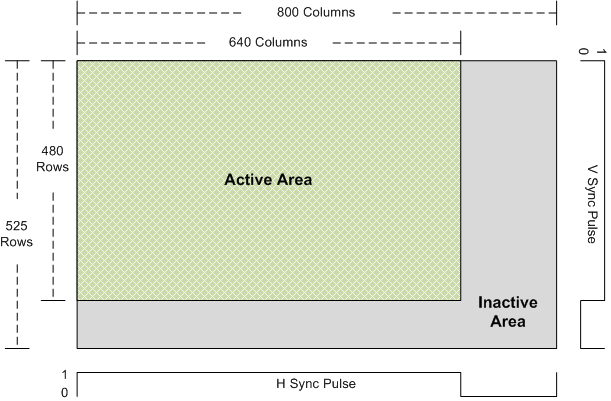
\includegraphics[width=0.8\textwidth]{vga-timing.png}
	\caption{VGA-Timing/Aufbau für eine 640x480 Auflösung, aus \cite{vga-timing}}
	\label{fig:vga}
\end{figure}

Eine 640x480 Pixel Bild baut sich dann wie in \autoref{fig:vga} gezeigt auf:
Zuerst werden 640 Pixel RGB Daten für die erste Reihe empfangen, danach kommen 160 Pixel inaktiver Bereich ($\Rightarrow$ Porch). Das Ende dieses Bereiches wird durch das Ansteigen des low-aktiven Signal HSYNC signalisiert. Dieser Vorgang wird nun 480 mal wiederholt, bis das gesamte Bild übertragen wurde. Draufhin wird analog zur horizonalen Synchronisation das VSYNC Signal für 45 Pixel auf auf 0 gesetzt, um den vertikalen inaktiven zu signalisieren. Die Länge des inaktiven Bereiches setzt sich aus Front-, bzw. Backporch und der Länge des Sync-Pulses zusammen. Die Bedeutungen der einzelnen Signale können fügen jedoch dem nötigen Verständnis nicht mehr hinzu, weswegen die Summe dieser Bereiche als Ganzes angesehen werden kann.
Wie schon erwähnt ist 640x480 jedoch nicht die einzige Auflösung, die mit einem VGA-Anschluss realisierbar ist. Andere Auflösungen (mit anderen Widerholungsraten) müssen vom verwendeten Bildschirm unterstützt sein, und werden durch verschieden schnelle Pixelclocks und Porches realisiert.\\
Die in dieser Arbeit verwendete Auflösung von 800x600 Pixeln bei 60Hz benötigt die in \autoref{tab:vga-timings} dargestellten Werte.

\begin{table}[H]
	\centering
	\begin{tabular}{|l|c|r|}	
		\hline
		aktiver Bereich (horizontal) & Pixel & 800 \\ \hline
		aktiver Bereich (vertikal) & Pixel & 600 \\ \hline
		inaktiver Bereich (horizontal) & Pixel & 256 \\ \hline
		inaktiver Bereich (vertikal) & Pixel & 28 \\ \hline
		Pixelfrequenz & MHz & 40 \\ \hline
	\end{tabular}
	\caption{VGA-Werte für ein 800x600@60Hz Signal}
	\label{tab:vga-timings}
\end{table}

Die in \autoref{tab:vga-timings} gezeigte Pixelfrequenz von 40 MHz bedeutet, dass alle 25 ns ein neuer RGB-Wert anliegen muss. Dies ist ein wichtiger Aspekt für weitere grundliegende Designentscheidungen. %TODO späteres Kapitel hier

\chapter{Theoretische Grundlagen}
Die dieser Arbeit zugrundelegenden mathematischen Grundlagen und Definitionen sollen in diesem Kapitel näher erläutert werden.

\section{Fraktale}
%todo mandelbrot pole/franz
Der Begriff \textit{Fraktal} wurde vom französischen Mathematiker Benoît Mandelbrot geprägt und leitet sich vom lateinischen Adjektiv \textit{fractus} ab, was \glqq in Stücke gebrochen\grqq{} oder \glqq irregulär\grqq{} bedeutet. Allgmein ist hiermit entweder eine natürlich vorkommende Strukur mit gewissen Eigenschaften oder eine genau definierte mathematische Menge gemeint. \cite[S. 16]{mandelbrot2013fraktale}\\
Für ein intuitives Verständnis des Begriffes sollen im folgenden zuerst einige natürlich vorkommende Fraktale gezeigt werden, woraufhin im nächsten Abschnitt eine formale Definition des Begriffs \textit{Fraktal} folgen soll.

\subsection{Natürlich vorkommende Fraktale}
\label{sec:natfrac}
Fraktale besitzen oft selbstähnliche Strukturen, d.h. dass sich die Gesamtstruktur eines Objektes in kleinerem Maßstab immer wieder findet. Ein Beispiel hierfür ist ein fraktal definierter Baum wie er in \autoref{fig:tree} dargestellt ist. Der Baum wird hierbei über ein einfaches rekursives Verfahren definiert, bei dem immer wieder von jedem Teilbaum aus mit einem festen Winkel in jeweils zwei Äste abgebogen wird.

\begin{figure}[H]
	\centering
	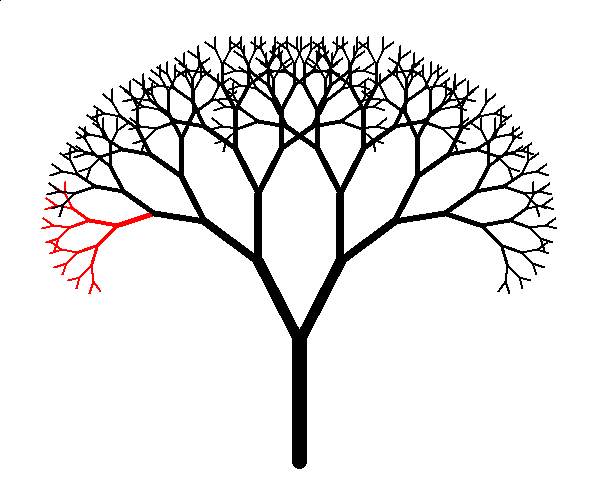
\includegraphics[width=0.6\textwidth]{tree.png}
	\caption{Fraktal definierter Baum, Skript: \textit{baum.py}, abgewandelte Version von \cite{soTree}} %TODO: Skript hinzufügen
	\label{fig:tree}
\end{figure}

Der in \autoref{fig:tree} rot markierte Teilbaum ist in seiner Struktur mit dem Gesamtbaum identisch und besitzt lediglich eine niedrigere rekursive Tiefe.\\
Der Blumenkohl (\autoref{fig:blumenkohl}) ist ein weiteres Beispiel für ein natürlich vorkommendes Fraktal. 
Auch bei diesem wiederholt sich die Gesamtstruktur in kleinerem Maßstab in den Ästen, er besitzt also ein gewisses Maß an Selbstähnlichkeit.

\begin{figure}[H]
	\centering
	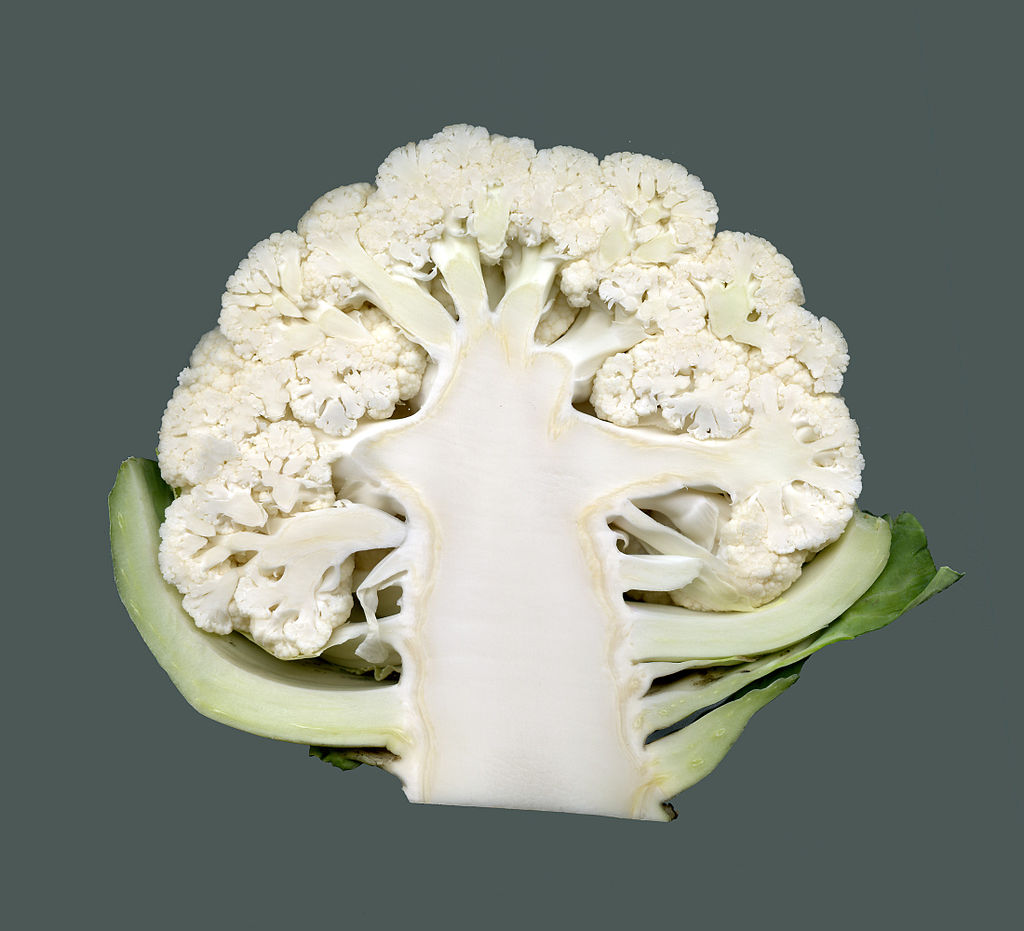
\includegraphics[width=0.4\textwidth]{blumenkohl}
	\caption{Blumenkohl, von Rainer Renz}
	\label{fig:blumenkohl}
\end{figure}

Auch auf höheren Maßstäben, wie etwa bei Bergen oder ganzen Landschaften können Fraktale Strukturen immer wieder beobachtet werden. 
Die relativ einfachen Regeln, die diesen Fraktalen zu Grunde liegen machten sich bereits im Jahre 1980 Computergrafiker wie etwa Loren Carpenter zu Nutzen. Die relativ begrenzten Rechnerleistungen zwangen Animatoren zu diesem Zeitpunkt dazu, komplexe Landschaften Bild für Bild von Hand zu zeichnen. Durch Mandelbrot's Arbeit in fraktaler Geometrie inspiriert animierte Carpenter eine Landschaft für den Film \textit{Star Trek II: The Wrath of Khan}, wobei er hierfür fraktale Verfahren verwendete. \cite{startrekFractals}\\
Die hierfür angestellten Berechnungen waren so simpel, dass pro Bildpunkt nur etwa 20 bis 40 Minuten Rechenaufwand betrieben werden mussten, was einen großen Fortschritt gegenüber der manuellen Animation darstellte. \cite{carpenterVolLibre}\\

\subsection{Fraktale in der Mathematik}
Im Gegensatz zu den in \autoref{sec:natfrac} dargestellten Fraktalen, welche sich auf kleinerer Ebene nur wenige male wiederholen, sind Fraktale in der Mathematik bis zu unendlich hohem Detailgrad definiert.\\
Die formale Definition eines Fraktals lautet hierbei nach Mandelbrot:

\begin{quotation}
	\textit{Ein Fraktal ist nach Definition eine Menge, deren  Hausdorff-Besicovitch Dimension echt die topologische Dimension übersteigt.}
	\\ - Benoît Mandelbrot, aus \cite[S. 27]{mandelbrot2013fraktale}
\end{quotation}
Die hier erwähnte Hausdorff-Besicovitch Dimension ist ein Maß, welches einem beliebigen geometrischen Raum zugeordnet werden kann, wobei die Dimension hier keine natürliche Zahl sein muss. In vereinfachter Form ermittelt sich die Hausdorff-Dimension folgendermaßen:\\
Man betrachte die Anzahl Kugeln (oder Kreisen) $N$ mit Radius $R$, die nötig sind, um eine Punktmenge vollständig abzudecken.
Geht nun $R$ gegen 0 werden immer mehr Kugeln benötigt, um die Punktmenge abzudecken. Beobachtet wird nun in welcher Relation $N$ zu $R$ wächst, mit Hilfe der Formel:
\[D = - \lim_{R \to 0} \frac{\log{N}}{\log{R}}\]
wobei D die Hausdorff-Dimension ist. Betrachtet man etwa eine Linie der Länge 1, kann diese zunächst mit $N = 1$ Kreisen des Radius $R = 1$ abdecken. Halbiert man nun $R$ sind doppelt so viele Kreise nötig um die Linie abzudecken. Allgemein lässt sich sagen, dass in diesem Fall $N$ umgekehrt proportional zu $R$ wächst. Drückt man nun $N$ in abhängigkeit von R aus erhält man für die Dimension einer Kurve:
\[D = - \lim_{R \to 0} \frac{\log{\frac{1}{R}}}{\log{R}} = 1\]
Analog werden etwa bei einem Rechteck $1/R^2$ Kugeln zur Abdeckung benötigt, wenn $R$ gegen 0 läuft. Die Dimension eines Rechtecks ist daher:
\[D = - \lim_{R \to 0} \frac{\log{\frac{1}{R^2}}}{\log{R}} = 2\]
Bei den hier gezeigten Formen ist die Hausdorff Dimension nicht höher als deren topolosche Dimension \footnote{s. hierzu \url{https://www.math.tu-cottbus.de/~froehner/sonstiges/skripte/node9.html}} 
Nimmt man jedoch nun ein Fraktal, wie etwa das Sierpinski-Dreieck %TODO vllt erklären
herbei, hat dieses oft einen gebrochenen Dimensionwert, in diesem Fall:
\[\frac{\log{3}}{\log{2}}\approx 1.585\]
Zusätzlich zu der bereits gezeigten Definition gilt:
Jede Menge, die einen nichtganzzahligen Dimensionwert hat, ist ein Fraktal\cite[S. 27]{mandelbrot2013fraktale}.

\section{Die Mandelbrotmenge}
Nachdem nun die formale Definition eines Fraktales bekannt ist, soll im folgenden Mandelbrotmenge erläutert werden.\\
Es gilt: Teil der Menge sind alle komplexen Zahlen $c$, für die die Iteration
\[z_0=0\]
\[z_{n+1}=z_n^2 + c\]
nicht divergiert.
Im folgenden sind Iterationen für einige $c$ gezeigt:
\[c_1=1 ; z=2 \rightarrow 5 \rightarrow 26 \rightarrow 677\]
\[c_2=-1 ; z=0 \rightarrow -1 \rightarrow 0 \rightarrow -1\]
\[c_3=1+1i ; z=1+3i \rightarrow -7+7i \rightarrow 1-97i \rightarrow -9407-193i\]

Für $c1$ und $c3$ sieht man schnell, dass der Betrag dieser Zahlen divergiert, während es bei $c2$ klar ist, dass $z$ nur zwischen 0 und -1 wechselt. Also ist $c2$ Teil der Menge, während es $c1$ und $c3$ nicht sind. Jedoch ist die Divergenz nicht für alle Werte so einfach festzustellen. Man betrachte folgendes $c$:
\[c_4=-0.55 + 0.46i ; z=0.45 - 0.04i \rightarrow -0.34 + 0.05i \rightarrow -0.68 + 0.11i \rightarrow -0.09 + 0.29i\]
Hier ist es zunächst unklar ob eine Divergenz stattfinden wird, es müssten erst viele Iterationsschritte angestellt werden, um eine Aussage treffen zu könnnen. Nach 200 Schritten ergibt sich die in \autoref{fig:mandel_c4} gezeigte Struktur, bei der man erkennen kann, dass $z$ gegen einen bestimmten Punkt konvergieren zu scheint.

\begin{figure}[H]
	\centering
	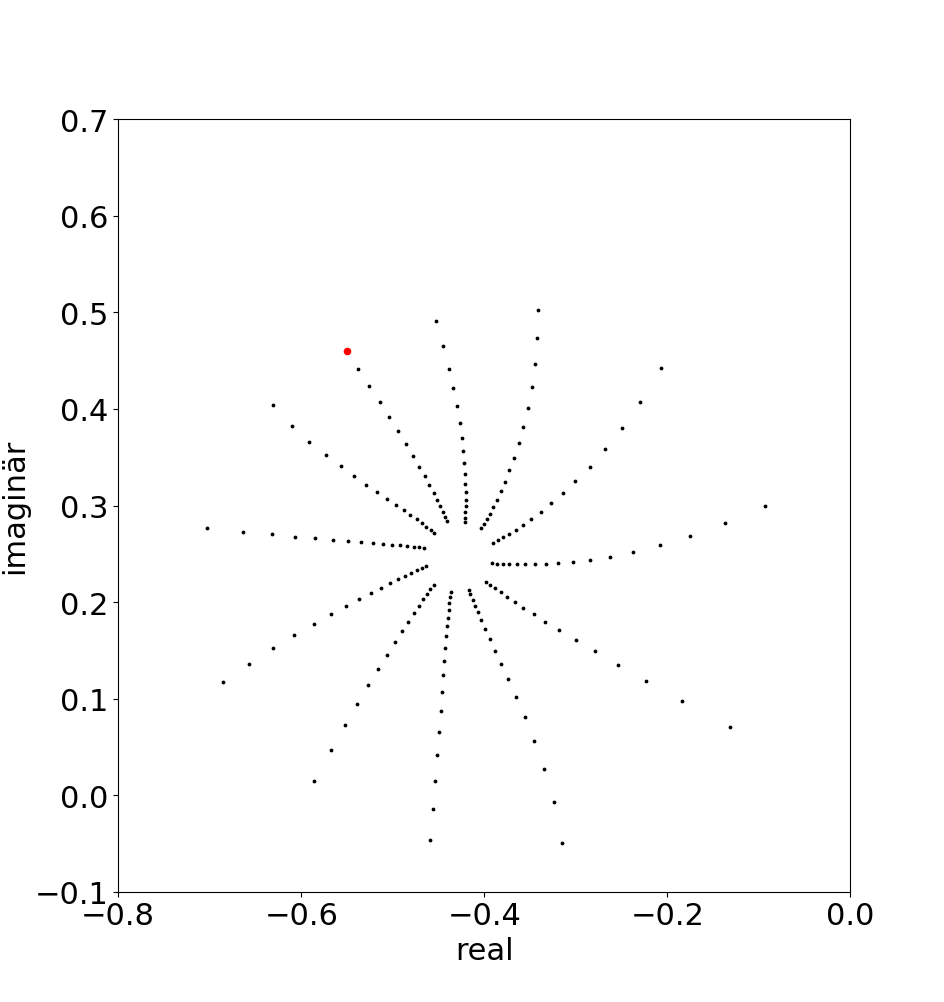
\includegraphics[width=0.6\textwidth]{mandel_c4.png}
	\caption{200 Iterationsschritte für $c = -0.55 + 0.46i$}
	\label{fig:mandel_c4}
\end{figure}

\chapter{Test und Umsetzung}
	\section{Gesamtsystem}
	\section{Komponentenbeschreibung}
		\subsection{Mandelbrot-Core}
		\subsection{Mandelbrot-Koordinator}
		\subsection{Dual Port Block RAM}
		\subsection{Lookup Tables}
	\section{Peripherie und funktionale Beschreibung}

\chapter{Optimierungen}
	\section{Algebraische Optimierung}
	\section{Designoptimierungen}

% Literaturverzeichnis
\bibliography{bib}{}
\bibliographystyle{unsrt}

\end{document}